% LaTex Table of Contents, Figures, and Tables example
\documentclass[11pt]{article}
\usepackage{fullpage}
\usepackage{graphicx}
\usepackage{hyperref}

%opening
\title{Lab 8 LaTex Table of Contents, Figures, and Tables}
\author{Jericho McLeod}

\begin{document}

\maketitle

\begin{abstract}
In this lab, we use LaTex features for automatically creating table of contents, figures, and tables.
\end{abstract}

\tableofcontents
\listoffigures
\listoftables
\newpage

\section{Iceland}
Iceland has become a popular tourist destination in recent years. 

\newpage %forces a new page
\section{Iceland  Map}
Here is a map of Iceland, showing the larger cities and the major highway that circumnavigates the island (see figure \ref{fig:IcelandMap}).
\begin{figure}[h!]
	\centering
	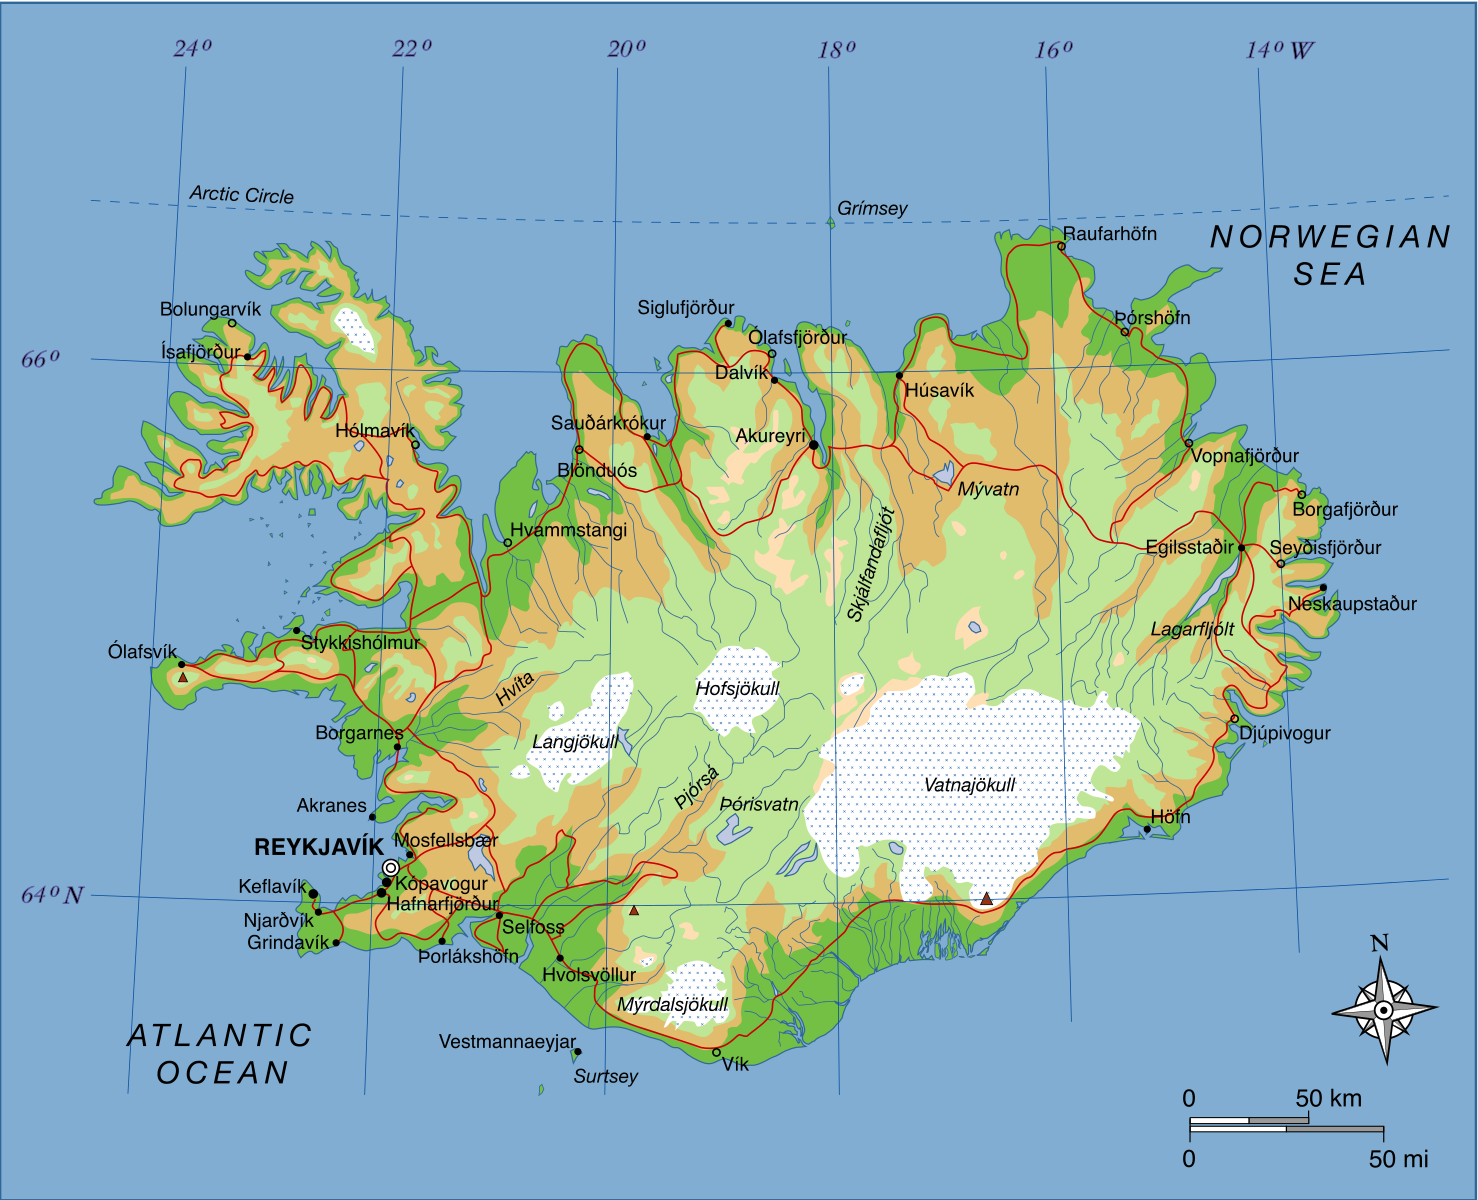
\includegraphics[width=0.7\linewidth]{Map_of_Iceland.png}
	\caption{Map of Iceland}
	\label{fig:IcelandMap}
\end{figure}

Source: \url{https://commons.wikimedia.org/wiki/File:Map_of_Iceland.svg}

\newpage
\section{Visitor Statistics}
Located at a convenient location for Trans-Atlantic flights to have layovers, Iceland now sees more than two million visitors per year (see Table \ref{tab:IcelandVisitorStats})

\begin{table}[h!]
\center
	\begin{tabular}{|c|r|}
		\hline
		Year & Visitors\\
		\hline
		2010 & 459,252\\
		\hline
		2011 & 540,824\\
		\hline
		2012 & 646,921\\
		\hline
		2013 & 781,016\\
		\hline
		2014 & 969,181\\
		\hline
		2015 & 1,261,938\\
		\hline
		2016 & 1,767,726\\
		\hline
		2011 & 2,195,271\\
		\hline
	\end{tabular}
	\caption{Iceland Annual Visitors, 2010-2017}
	\label{tab:IcelandVisitorStats}
\end{table}

Source: 
\href{https://www.ferdamalastofa.is/is/um-ferdamalastofu/frettir/22-milljonir-erlendra-farthega-2017}{https://www.ferdamalastofa.is}

\newpage
\section{Waterfalls}
Iceland is known for its vast number of waterfalls. Here is a limited selection of them (see Figures \ref{fig:skogafoss} and \ref{fig:seljalandsfoss}).

\begin{figure}[h!]
	\centering
	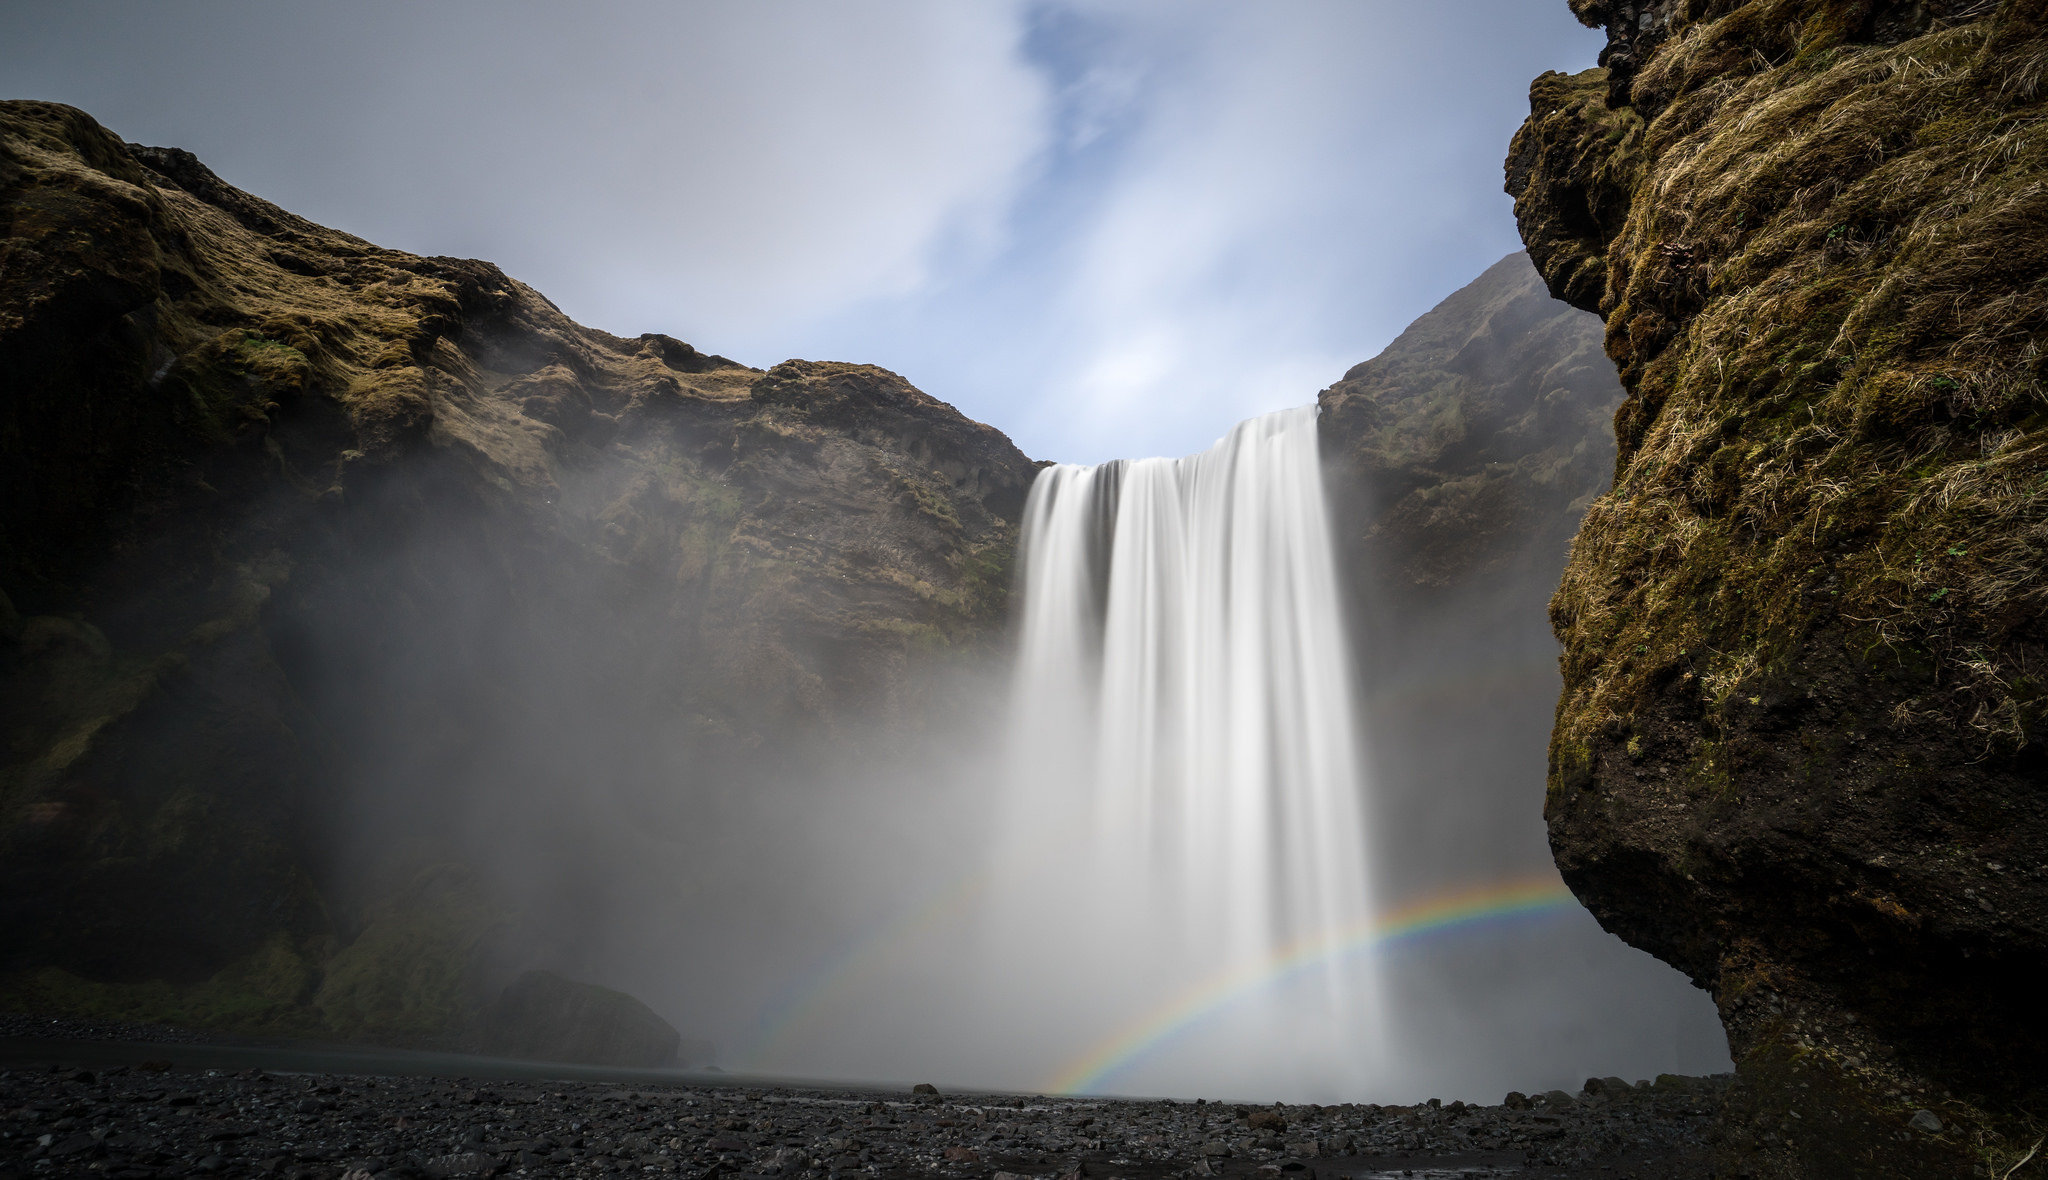
\includegraphics[width=0.7\linewidth]{skogafoss.jpg}
	\caption{Sk\'ogafoss (The Forest Waterfall) by Jericho McLeod, 2018 \textcopyright}
	\label{fig:skogafoss}
\end{figure}

\begin{figure}[h!]
	\centering
	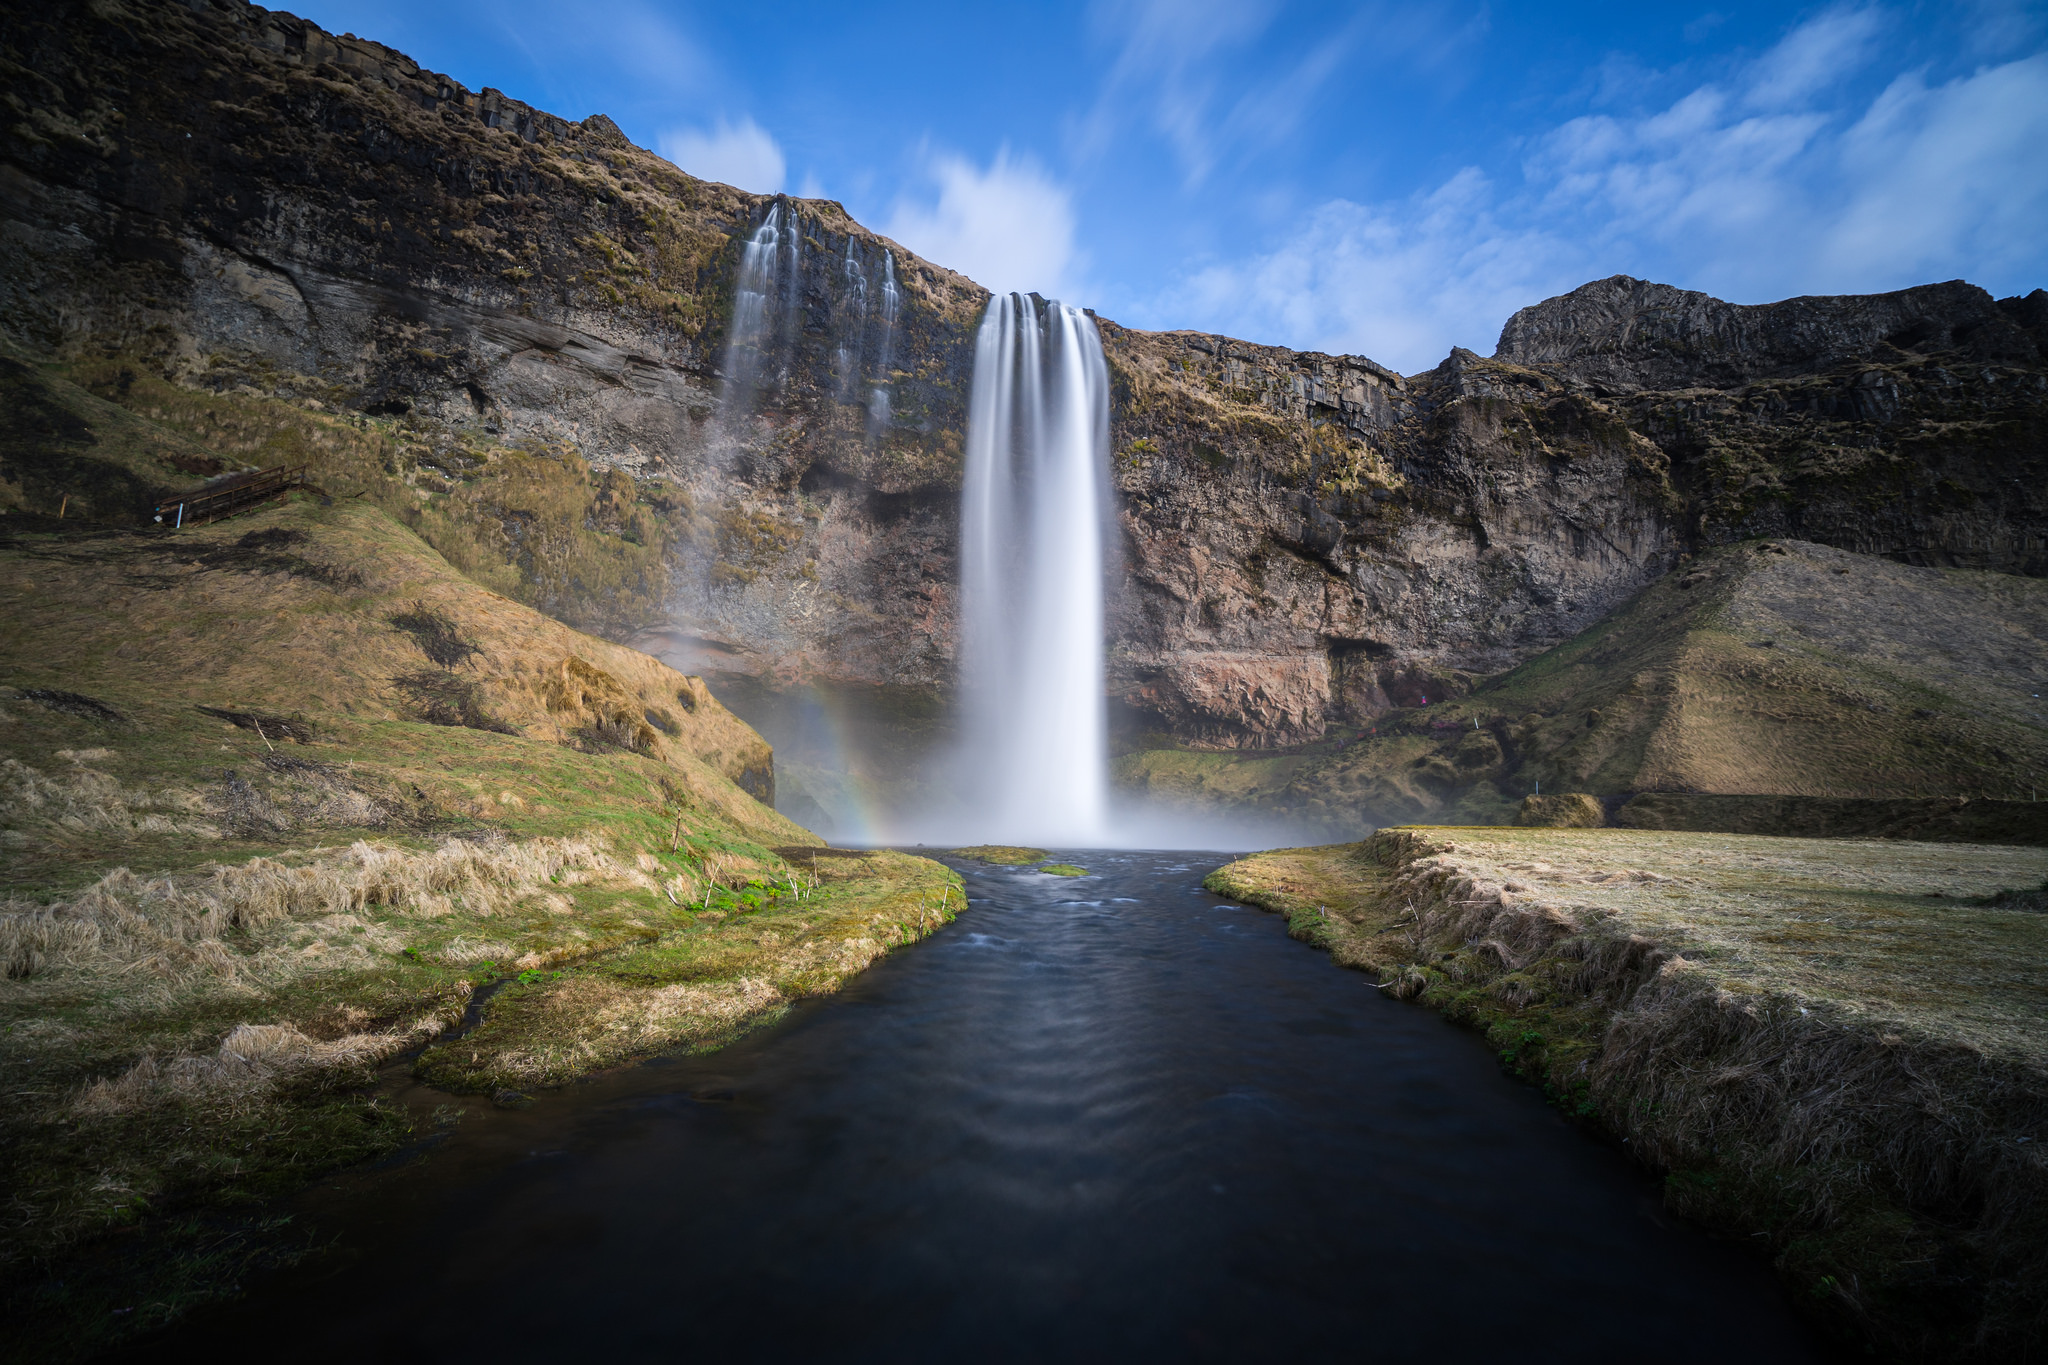
\includegraphics[width=0.7\linewidth]{seljalandsfoss.jpg}
	\caption{Seljalandsfoss (Selling the Land of Waterfalls) by Jericho McLeod, 2018 \textcopyright}
	\label{fig:seljalandsfoss}
\end{figure}



\end{document}
